\section{Introduction}

\begin{description}
\item[Problem]

Nowadays, people, business and every single device becomes a data factory that generates data. Billions of internet users turn the data quality to interesting and important area for researcher.In one hand data quality getting more important in the industry because this valuable process, can help companies to save time,money and let them to increase their efficiency.On the other hand, scientific researchers use clean version of datasets for their discoveries,approach and researches.In this regard,always custom error generator has been wanted by researchers to let them make new datasets out of one dataset,with fully control on amount and type of errors.

\felix{Many machine learning applications today are based on user data. For instance, user add products, their descriptions, and ratings to Amazon. Amazon trains on this user-entered data machine learning models to recommend products and estimate prices. Users are humans and therefore make mistakes. These mistakes can harm machine learning models. Therefore, for data scientists, it is essential to know whether and to which degree their feature representation and models are robust against a wide range of possible user errors.}

\milad{Nowadays, people, business and every single device becomes a data factory that generates data.At the same time, Many machine learning applications are based on user data.For instance, user add products, their descriptions, and ratings to Amazon. Amazon trains on this user-entered data machine learning models to recommend products and estimate prices. Users are humans and therefore make mistakes. These mistakes can harm machine learning models.As result, data quality turns to interesting and important area for researcher.in this regard, it is essential to know whether and to which degree their feature representation and models are robust against a wide range of possible user errors
}


Dirty Fire as first custom error generator that provides user ability to control accuracy and it can provide errors that does not influence the accuracy and even help more by finding the weakness of machine learning models and corresponding feature representations.Dirty fire have ability to make this flow cheaper by adding several type of errors that have more influence on the models.



\item[why interesting?] 
Dirty Fire let the user to check the robustness of machine learning models and with cheap operation cost find the weakness of the models.
\item[why hard?]
recursive task that Dirty Fire check each time the effects of the changes on the accuracy are expensive. \felix{not only accuracy: be more general: cost metric}
\milad{calculate the level of robustness of the model against the error and recursively update that, increase the cost metric and control the cost metric as same as efficiency is the main contribution of this paper.}
\vspace{2mm}

\milad{Motivation example:let's assume there is the dataset with the 165 data points and regarding the binary classification we have got the above result(Fig.1)
as we already know from the figure1 TN=50, TP=100, FP=10, FN=5 ,Accuracy=0.9.Dirty Fire can change the data set with the order to balance of TP+TN would remain the same which is mean we have another dataset with the same accuracy or it let's user to generate the error with fully control on confusion matrix }
\vfill

\begin{figure}
	\centering
	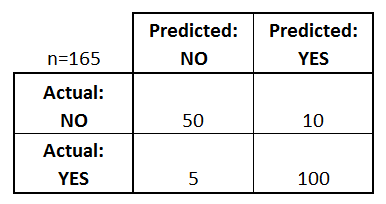
\includegraphics[width=0.3\textwidth]{img/motivation1.png}
	\caption{Motivation Example}
	\label{figure:Motivation Example}
\end{figure}



\end{description}

\begin{figure*}[ht!]
	\centering
	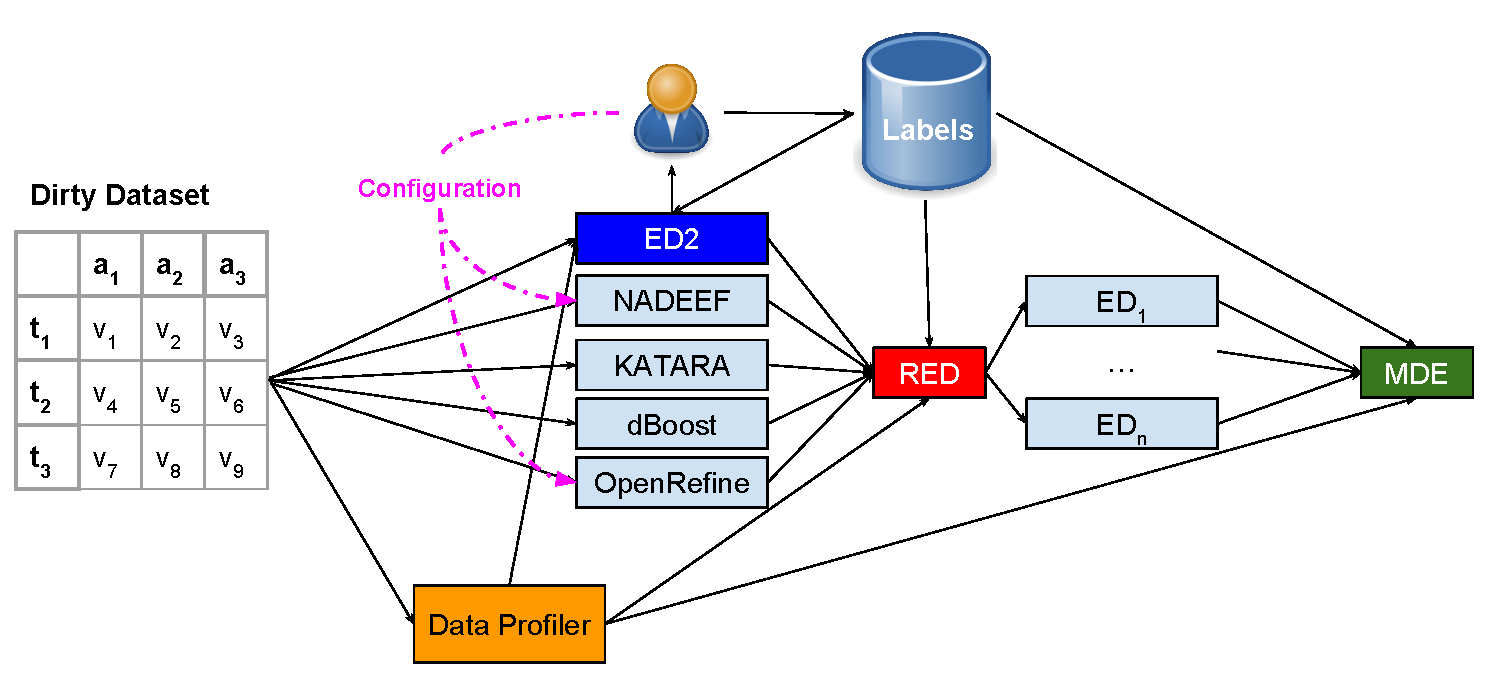
\includegraphics[width=0.9\textwidth]{img/demo.pdf}
	\caption{Architecture.}
	\label{figure:architecture}
\end{figure*}
